%%%%%%%%%%%%%%%%%%%%%%%%%%%%%%%%%%%%%%%%%%%%%%%%%%%%%%%%%%%%%%%%%%%%%%%%%%%%%%%%%%%%%%%%%%%%%%%%%%%%%%%%%%%%%%%%%%%%%%%%%%%%%%%%%%%%%%%%%%%%%%%%%%%%%%%%%%%
% This is just an example/guide for you to refer to when submitting manuscripts to Frontiers, it is not mandatory to use frontiers.cls nor frontiers.tex  %
% This will only generate the Manuscript, the final article will be typeset by Frontier after acceptance.                                                 %
%                                                                                                                                                         %
% When submitting your files, remember to upload this *tex file, the pdf generated with it, and all the figures.
%%%%%%%%%%%%%%%%%%%%%%%%%%%%%%%%%%%%%%%%%%%%%%%%%%%%%%%%%%%%%%%%%%%%%%%%%%%%%%%%%%%%%%%%%%%%%%%%%%%%%%%%%%%%%%%%%%%%%%%%%%%%%%%%%%%%%%%%%%%%%%%%%%%%%%%%%%%

%%% Version 2.4 Generated 2014/03/12 %%%
%%% You will need to have the following packages installed: datetime, fmtcount, etoolbox, fcprefix, which are normally inlcuded in WinEdt. %%%
%%% In http://www.ctan.org/ you can find the packages and how to install them, if necessary. %%%

%\documentclass{frontiersENG} % for Engineering articles
\documentclass{frontiersSCNS} % for Science articles
%\documentclass{frontiersHLTH} % for Health articles
%\documentclass{frontiersFPHY} % for Physics articles

\setcitestyle{square}
\usepackage{url,lineno}
\linenumbers

\usepackage[hidelinks]{hyperref}
\usepackage{ucs}
\usepackage{pbox}
%\usepackage{inputenc}
\usepackage{amsmath,amssymb,amstext}
\usepackage{graphicx}
\usepackage{graphics}
\usepackage{caption}
%\usepackage[automark]{scrpage2}
%\pagestyle{scrheadings}
%\usepackage{appendix}
%\usepackage[nottoc,numbib]{tocbibind}

%\usepackage{synttree}
%package{pgf}
%\usepackage{tikz}
%\usepackage{multicol}
\usepackage{gensymb}
%\usepackage{hyperref}
%\bibliographystyle{plainnat}
%\usepackage[authoryear]{natbib}
%\citestyle{nature}
%\bibpunct{(}{)}{;}{a}{:}{,}


\graphicspath{{figures}}


% Leave a blank line between paragraphs in stead of using \\

\copyrightyear{}
\pubyear{}

\def\journal{Behavioral Neuroscience}%%% write here for which journal %%%
\def\DOI{}
\def\articleType{Research Article}
\def\keyFont{\fontsize{8}{11}\helveticabold }
\def\firstAuthorLast{Kitson {et~al.}} %use et al only if is more than 1 author
\def\Authors{Alexandra Kitson,$^{1,*}$, Daniel Sproll\,$^{2}$ and Bernhard E. Riecke,$^1$}
% Affiliations should be keyed to the author's name with superscript numbers and be listed as follows: Laboratory, Institute, Department, Organization, City, State abbreviation (USA, Canada, Australia), and Country (without detailed address information such as city zip codes or street names).
% If one of the authors has a change of address, list the new address below the correspondence details using a superscript symbol and use the same symbol to indicate the author in the author list.
\def\Address{$^{1}$School of Interactive Arts + Technology, Simon Fraser University, Surrey, BC, Canada \\
$^{2}$Institute of Cognitive Science, University of Osnabr\"uck, Germany }
% The Corresponding Author should be marked with an asterisk
% Provide the exact contact address (this time including street name and city zip code) and email of the corresponding author
\def\corrAuthor{corresponding Author}
\def\corrAddress{Alexandra Kitson, School of Interactive Arts + Technology, Simon Fraser University, Surrey, BC, Canada.}
\def\corrEmail{akitson@sfu.ca}

% \color{FrontiersColor} Is the color used in the Journal name, in the title, and the names of the sections.


\begin{document}
\onecolumn
\firstpage{1}

\title[Individual Factors in Path Integration]{Influence of Ethnicity, Gender and Answering Mode on a Virtual Point-to-Origin Task}
\author[\firstAuthorLast ]{\Authors}
\address{}
\correspondance{}
\extraAuth{}% If there are more than 1 corresponding author, comment this line and uncomment the next one.
%\extraAuth{corresponding Author2 \\ Laboratory X2, Institute X2, Department X2, Organization X2, Street X2, City X2 , State XX2 (only USA, Canada and Australia), Zip Code2, X2 Country X2, email2@uni2.edu}
\topic{}% If your article is part of a Research Topic, please indicate here which.

\maketitle

%%%%%%%%%%%%%%%%%%%%%%%%%%%%%%%%%%%%%%%%%%%%%%%%%%%%%%%%%%%%%%%%%%%%%%%%%%%%%%%%%%%%%%%%%%%%%%%%%%%%%%%%%%%%%%%%%%%%%%%%%%%%%%%%%%%%%%%%%%%%%%%%%%%%%%%%%%%%%%%%%%%%%%%%%%%%%%%%%%%%%%%%%%%%%%%%%%%%%%%%%%%%%%%%%%%%%%%%%%%%%%%%%%%%%%%
%%% The sections below are for reference only.
%%%
%%% For Original Research Articles, Clinical Trial Articles, and Technology Reports the section headings should be those appropriate for your field and the research itself. It is recommended to organize your manuscript in the
%%% following sections or their equivalents for your field:
%%% Abstract, Introduction, Material and Methods, Results, and Discussion.
%%% Please note that the Material and Methods section can be placed in any of the following ways: before Results, before Discussion or after Discussion.
%%%
%%%For information about Clinical Trial Registration, please go to http://www.frontiersin.org/about/AuthorGuidelines#ClinicalTrialRegistration
%%%
%%% For Clinical Case Studies the following sections are mandatory: Abstract, Introduction, Background, Discussion, and Concluding Remarks.
%%%
%%% For all other article types there are no mandatory sections.
%%%%%%%%%%%%%%%%%%%%%%%%%%%%%%%%%%%%%%%%%%%%%%%%%%%%%%%%%%%%%%%%%%%%%%%%%%%%%%%%%%%%%%%%%%%%%%%%%%%%%%%%%%%%%%%%%%%%%%%%%%%%%%%%%%%%%%%%%%%%%%%%%%%%%%%%%%%%%%%%%%%%%%%%%%%%%%%%%%%%%%%%%%%%%%%%%%%%%%%%%%%%%%%%%%%%%%%%%%%%%%%%%%%%%%%

\begin{abstract}

%%% Leave the Abstract empty if your article falls under any of the following categories: Editorial Book Review, Commentary, Field Grand Challenge, Opinion or specialty Grand Challenge.
\section{}
%As a primary goal, the abstract should render the general significance and conceptual advance of the work clearly accessible to a broad readership. References should not be cited in the abstract.
%Refer to \\ \url{http://www.frontiersin.org/}\texttt{\journal}\url{/authorguidelines} \\ or \textbf{Table\ref{Tab:01}} for abstract requirement and length according to article type.
The study investigated the turner and non-turner phenomenon reported in \citep{Klatzky1998}, \citep{Gramann2005},  and  \citep{Riecke2008} using a virtual point-to-origin task. There are three main goals of the study: replicate the gender effect found by \citep{Goeke2013}; extend the effect, found by  \citep{Avraamides2004}, of higher turner numbers with spatial language, opposed to pointing, response mode; examine ethnicity influence on turner and non-turner behavior.
The experiment was designed as a classroom study with a high number of participants ($n=498$). We presented participants with four short passages through a virtual star field where, at the end, participants selected the direction pointing back to the origin from four multiple-choice items. There were two different response sheets: pictograms and written language. After the experiment, participants filled out a demographics questionnaire.
A majority of participants ($44.78\%$) was classified as non-turners, while $25.3\%$ were turners and $18.88\%$ had no preference. A multinomial regression model with variables, condition, and all interaction terms was fitted. Classification performance reached $49\%$, and two main factors (Ethnicity and Condition) and two interaction terms (Ethnicity: Condition and Condition: Gender) were significant. 
Odds ratios showed that written spatial language, compared to pictograms, made the turner strategy more likely. The effect was more pronounced for Chinese subjects and among females, and was not significant for male Caucasians. 
We extended the findings of \citep{Avraamides2004}, showing higher numbers of turners when using spatial language instead of pointing. Unlike \citep{Goeke2013}, influence of gender was not significant. We found that ethnicity has an influence on turner and non-turner behavior. Caucasians, especially males, are a special subpopulation when it comes to point-to-origin tasks in virtual environments, having a comparably high ratio of turners to non-turners.


\tiny
 \keyFont{ \section{Keywords:} spatial navigation, reference frames, path integration, navigational strategies, gender differences, ethnicity differences } %All article types: you may provide up to 8 keywords; at least 5 are mandatory.
\end{abstract}

\section{Introduction}

% For Original Research Articles, Clinical Trial Articles, and Technology Reports the introduction should be succinct, with no subheadings.
%
% For Clinical Case Studies the Introduction should include symptoms at presentation, physical exams and lab results.
%
%Spatial navigation: 
We are able to navigate and orient ourselves effortlessly through the world. Yet, when we put ourselves in a virtual world navigation becomes cognitively demanding. Why the discrepancy? Normally we rely on vision, audition, vestibular, and proprioceptive input to automatically guide us and update our position. We use two distinct reference frames: egocentric, self-to-object representation, and allocentric, object-to-object representation. We are forced to exclusively use our egocentric reference to navigate in the real world. Forming and maintaining spatial representations is hard to suppress, and ignoring it takes conscious cognitive effort \citep{Riecke2005}. Yet, when we imagine the same path, we tend to use a mixed strategy to determine where we are. During navigation, spatial representations are not only constantly updated and maintained in parallel but also interact \citep{Moser2008}. When exactly we use a specific reference frame for a certain task remains a difficult question because individual proclivities come into play \citep{Gramann2011}. 

Spatial navigation is a deep rooted and modularized cognitive skill based on spatial representations that are automatically formed and maintained (updated) in specialized brain areas based on multimodal sensory information. Different reference frames for spatial orientations seem to be processed in distinct neural correlates \citep{Gramann2010,Zaehle2007}. The sensory information from all senses is automatically combined into a spatial representation in the brain involving a wide network of brain regions (for a review see \cite{Moser2008}). However, there are times when spatial updating fails, especially when we receive incomplete or contradicting sensory information. In such cases, we revert to offline strategies where we try to cognitively restore our spatial representations. These offine strategies enable researchers to study the mechanism of spatial updating in more detail: when is spatial updating automatic and obligatory, and when does it brake down? What factors decide which reference frame we use for our spatial representation? 

%Spatial strategies: 
Researchers have discovered a phenomenon involving spatial updating and spatial representations in different reference frames \citep{Klatzky1998} where, in a point-to-origin paradigm, participants experienced a virtual visual flow environment. Here, the “turner” group used an egocentric reference frame updated during the trajectory and the “non-turner” group responded as if they were still facing the original direction they started. However, those using the “non-turner” strategy solved the task correctly based on their strategy, applying an allocentric reference frame that stays constant throughout the trajectory.
%VR/VE: 
The advent of virtual reality (VR) technology gave researchers the opportunity to create experiments where the availability and fidelity of visual, vestibular, proprioceptive and auditive information channels can be controlled separately in a highly controlled way. This enables researchers to systematically dissociate the different influences of the modalities on complex tasks like spatial navigation.

%Individual factors and related works: 
Previous studies have looked at the individual factors that may influence the strategy used for spatial updating in a virtual point-to-origin task, such as gender, video gaming experience, ethnicity, response mode, navigation skills, cardinal direction proficiency, and decision certainty \citep{Goeke2013,Avraamides2004,Riecke2008}. 
% Gramanns theory
Gramann hypothesized that non-turners respond as if they had not turned and are still facing the original direction. Participants solved the task in a more abstract and disembodied way, applying an allocentric reference frame that stayed constant during the passage. Thus, what was thought to be an error in solving the task turned out to be a different strategy, where the answer is expressed in a different reference frame.
% Avraamides study
\citep{Avraamides2004} showed that an increased error (corresponding to non-turner behaviour) did not arise when participants performed an imagined triangle completion task and answered using spatial language instead of pointing. The researchers concluded that the non-turner answers in the pointing condition are due to the strong attachment of the pointing gesture to the current perceived body position, that is,  aligned with the hypothetical allocentric reference frame. 

% Avraamides vs Gramann
Avraamides' hypothesis is notably different from the one used by Gramann. While they both agree that participants giving turner answers update their egocentric reference frame according to the given stimulus (i.e., imaginary walking, visual flow, etc.), they have different explanations for the non-turner answers. Gramann explains non-turner behaviour as a different strategy of solving the task using an allocentric reference frame. Avraamides sees non-turner answers as an artifact of the task, namely the conflict between a virtual body orientation and a physical body orientation. Here, non-turner answers are not valid answers in an allocentric reference frame but errors due to an overriding of the virtual egocentric reference frame with a physical egocentric reference frame. However, he found this conflict is not present when spatial language is used to give the answers. Avraamides explains non-turner behaviour with a more abstract and less embodied nature of spatial language compared to bodily pointing; this strategy might be closer to a more cognitive representation of heading.
% careful language
To enable a neutral discussion of the phenomenon, in this study we will use the terms turner and non-turner referring only to behavioural observation - whether participants incorporated the virtual turn in their response or not without making an implicit assumption of which reference frame they use.

% more turner bla
Several other studies (see Table \ref{tab:01}) have investigated individual factors determining strategy selection, but no coherent picture has emerged. Individual proclivities seem to have a significant influence on strategy selection \citep{Gramann2011}, so we may be able to observe similar influences for automatic spatial updating, e.g., a more prominent use of a turner strategy in studies with naturalistic scenes and vestibular input \citep{Sigurdarson}. 
% Goecke study
The first big cross-sectional study investigating the turner and non-turner phenomenon was an online study conducted by \citep{Goeke2013}. Their sample contained (after preprocessing) 260 participants from 15 countries, with the majority from Spain and Germany. The task contained left right (yaw) turns as well as up and down turns (pitch). Answers were given via selecting one of four 3D arrows. In their analysis they found the factors gender, cardinal direction proficiency and decision certainty to be significant factors determining turner and non-turner behaviour, though this was not the case for self-estimated general navigation skills or video gaming experience. Overall, it seems that a multitude of known and unknown factors influence strategy use, leading to partially widely varying ratios of turners to non-turners in different studies.

% Ethnicity
One factor yet to be investigated is potential infuence of ethnicity on virtual navigation strategy. A large body of literature has well established the link between culture and cognitive style \citep{kitayama2010,kitayama2009,norenzayan2007,varnum2008}. Western cultures, such as the United States, tend to exhibit a more independent and analytic social orientation: “emphasizing uniqueness, having relatively low sensitivity to social cues, and encouraging behaviours that affirm autonomy”. On the other hand, other cultures such as China tend to exhibit a more interdependent and holistic social orientation: “emphasizing harmonious relations with others, promoting sensitivity to social cues, and encouraging behaviours that affirm relatedness to others” \citep{kitayama2010,varnum2010}. On the basis of such evidence, the link between social orientation and cognitive style has been widely accepted. \citep{Goeke2013} suggest looking at “cultural background on reference frame proclivity to finally unravel the underlying factors determining human navigation strategies.”

\begin{table}[h!]
\textbf{\refstepcounter{table}\label{tab:01} Table \arabic{table}.}{ An overview over turner studies, the used parameters and the percentage of turners ordered by the latter}
\begin{flushleft}
\resizebox{\textwidth}{!}{
\begin{tabular}{lll|ll|llllll|r}
	\multicolumn{3}{c}{ } & \multicolumn{2}{c}{\textbf{context}} & \multicolumn{6}{c}{\textbf{sensory information}}  & \multicolumn{1}{c}{} \\ 
	study & condition & n & answer & scene & visual & \pbox{2cm}{proprio-\\ceptive} & \pbox{2cm}{vesti-\\bular} & visual & \pbox{2cm}{horizontal\\resolution} & FOV & \multicolumn{1}{l}{\textbf{\pbox{2cm}{\% of \\turners}}} \\ \hline
\cite{Klatzky1998} & blind walking & 10 & point & blind & no & yes & yes & blind & 0 & 0 & \textbf{100} \\ 
\cite{Klatzky1998} & HMD \& Turn & 10 & point & starfield & yes & no & yes & HMD & 800 & 44x33 & \textbf{100} \\ 
\cite{Avraamides2004} & verbal  & 20 & describe & blind & no & no & no & blind & 0 & 0 & \textbf{100} \\
\cite{Riecke2007} & standard & 20 & point & plane & yes & no & no & Projector & 1400 & 84x63 & \textbf{45} \\ 
\cite{Sigurdarson} & real turn & 12 & point & naturalistic & yes & no & no & HMD & 800 & 32x24 & \textbf{83} \\ 
\cite{Sigurdarson} & visual turn & 12 & point & naturalistic & yes & no & yes & HMD & 800 & 32x24 & \textbf{83} \\ 
\cite{Riecke2008} & standard & 16 & point & ground plane & yes & no & no & Projector & 1400 & 84x63 & \textbf{62} \\ 
\cite{Riecke2008} & angle announced & 24 & point & ground plane & yes & no & no & Projector & 1400 & 84x63 & \textbf{54} \\ 
\cite{Plank2010} & standard & 37 & select & tunnel & yes & no & no & Projector & 800 & 41x41 & \textbf{54} \\ 
\cite{Gramann2010} & standard & 12 & select & tunnel & yes & no & no & Projector & ? & 41 & \textbf{52} \\
\cite{Gramann2012} & Experiment 2 & 11 & select & starfield & yes & no & no & Monitor & ? & 47x35 & \textbf{50} \\ 
\cite{Gramann2005} & all conditions & 43 & select & tunnel & yes & no & no & Monitor & ? & ? & \textbf{47} \\ 
\cite{Goeke2013} & online & 260 & select & starfield & yes & no & no & Monitor & 1024 & ? & \textbf{37} \\ 
\cite{Chiu2012} & standard & 20 & adjust & tunnel & yes & no & no & Projector & ? & 206 & \textbf{35} \\ 
\cite{Klatzky1998} & only HMD & 10 & point & starfield & yes & no & no & HMD & ? & 44x33 & \textbf{0} \\ 
\cite{Avraamides2004} & Imagine \& walk & 20 & turn & blind / real & yes & no & no & blind / real & 0 & 0 & \textbf{0} \\ 
\end{tabular}
}
\end{flushleft}
\label{tab:studyOverview}
\end{table}


%Goals of the Present Study
%In the following study we want to replicate the influence of parameters already in the model and add new facets.
We have three goals:
1. Replicate the gender bias found in \citep{Goeke2013}. We hypothesize, based on the literature, females are more likely to be non-turners compared to males.
2. Extend the findings of \cite{Avraamides2004}, predicting a higher amount of turners when spatial language, opposed to pointing, is used. We will use written spatial language vs. pictograms.
3. Investigate a possible influence of ethnicity on strategy selection.

To answer these three questions, we designed our study with the idea of having a very large sample size to cope with intrinsically noisy strategy classification data and high individual differences. We used a design that could be executed with many participants simultaneously, showing the stimulus on a projector and recording the answers via a paper questionnaire. This way, we were able to perform the experiment in lecture halls at the beginning of regular courses. We chose a small number of trials, since earlier studies have shown that strategies are relatively stable over time \citep{Goeke2013}. As a consequence of the study design, we could not directly employ the same answering modes as in \cite{Avraamides2004}. Instead, we used pictograms for the more embodied version and written spatial language for the equivalent of description on spatial language. We are aware that these answering modes are somewhat more abstract that the ones used by Avraamides and, thus, expect weaker effects.


%\begin{methods}
\section{Material \& Methods}

\subsection{Participants}
A total of 507 participants took part in the study: 228 female, 273 male, and 6 NA. Participants with missing gender or ethnicity data were cut out (n = 6). The average age was 20.5 years (SD = 3.2). We recruited a diverse spectrum of participants from 3 universities: Simon Fraser University (244 participants) and the University of British Columbia (183 participants) both in Vancouver, Canada, and the University of Osnabr\"uck in Germany (104 participants). An effort was made to recruit a sample with high ethnic diversity (see Fig. \ref{fig:01}). Participants were not reimbursed.
%\begin{table}[h]
%%\centering
%\resizebox{\columnwidth}{!}{%
%\begin{tabular}{c||c|c|c|c|c|c|c|c|c}
%	 & 	White 	&  Chinese 	& 				\multicolumn{7}{|c}{other}				\\ \cline{4-10}
%	 & & & \pbox{3cm}{East\\Asian} & \pbox{3cm}{South\\Asian} & \pbox{3cm}{Southeast\\Asian} & \pbox{3cm}{Middle\\Easter} & Black & \pbox{3cm}{Latin\\American} & other \\
%	\hline
%	total     & 117/70 & 87/92 & 13/17 & 11/8 & 15/12 & 10/7 & 3/0 & 6/3 & 11/19  \\			
%	\hline
%	pictorial & 62/41 & 58/56 & 					\multicolumn{7}{|c}{47/49}		 \\
%	\hline
%	textual   & 55/29 & 29/36 & 					\multicolumn{7}{|c}{22/17}								 
%\end{tabular}
%}
%\caption{}
%\end{table}

\subsection{Stimulus \& Apparatus}
Participants were shown a passage through a virtual starfield, providing optical flow without any landmarks. Trajectories consisted of an initial straight path, followed by a curve and a second straight path at the end. Curve angles used for the four trials were $60 \degree \ left$, $90 \degree \ right$, $90 \degree \ right$ and $60\degree \ left$, respectfully (paths are illustrated in Fig. \ref{fig:02}). The velocity profile was smoothed to make the stimulus less artificial and prevent nausea. The first linear part included a $1s$ linear acceleration phase with $10 \frac{m}{s^2}$, followed by a constant movement with $10 \frac{m}{s}$ for $2s$. The turn was divided into an accelerating half and a decelerating half, the constant acceleration being $15 \frac{\degree}{s^2}$, resulting in an overall turn time of $4s$ for $60 \degree$ and $5s$ for $90 \degree$. The second linear part consisted of a $3s$ constant linear movement and $1s$ deceleration -  slightly longer than the first part. 

Velocities and distances are abstract in a starfield environment and subjective perception highly depends on the starfield parameters chosen (star size, area and visibility range). Passages were programmed using \textit{Vizard 4.0}. Code for the pre-study can be found online (\url{http://github.com/leftbigtoe/starfield}) and can be executed with the free trial version of \textit{Vizard 4.0}.


% questionnaire
Answers were given via a multiple choice questionnaire (see supplemental material). For each trial of the point-to-origin task, the same four possible answers could be selected: front left, front right, back left, and back right for both the textual condition and the pictorial condition. For each trial, the sequence of items was randomized to avoid answering tendencies. The response form was folded and sealed with tape, with the demographic information questionnaire inside to prevent possible task performance bias. 
% projectors
The stimulus was shown on classroom projectors and lights were dimmed where possible. Participants were asked to group as closely as possible around the projector to minimize extreme viewing angles.

\subsection{Procedure}
The experiment took place either at the beginning or at the end of the classes. The lecturer introduced the experimenter, followed by distribution of informed consent forms. All students volunteering to participate signed the consent form and were randomly handed a pictorial or text condition response form. The experimenter then explained the task until no subject had further questions. Participants were asked to select the answers as quickly and intuitively as possible. They were also asked not to copy from their neighbours or discuss their answers until after the experiment.
Trials were shown to the class, pausing after each trial until everyone finished. No questions were answered that could provide feedback.
After completing the task, the room was illuminated again and participants were asked to open their forms and fill out the demographics questionnaire. In total, the experiment took approximately 10 minutes.

\subsection{Preprocessing}
Before the analysis, preprocessing was performed on the collected data. Only participants who provided data for ethnicity and gender, and had no missing answers for the navigation task were used ($n = 6$ participants excluded). For each trial, strategy was classified (turner, non-turner, frontal pointing 1 or frontal pointing 2), in accordance with previous studies (e.g., \cite{Goeke2013}), where participants were classified as users of the respective strategy based on consistent strategy use in $75\%$ of the trials. All others were classified with no preference. Frontal pointing 1 occurs when participants choose a response in the direction of the turn, and frontal pointing 2 occurs when participants choose a response in the opposite direction of the turn. Only three participants were classified as frontal pointing 2 users and, because no explanation could be given to this answering pattern, those answering patterns were considered to be due to inattentiveness. We excluded participants classified as frontal pointers 2 from further analysis due to sparseness of data ($n = 3$ participants excluded). Statistical analysis was performed with the remaining $n = 498$ participants.

\subsection{Data Analysis}
R 2.15.2 was used for data analysis. A multinomial regression model was used for statistical analysis and a likelihood ratio test of the parameters was done using an ANOVA.


%\end{methods}



\section{Results \& Discussion}

\subsection{General Response Behaviour}


% pref strat
Total counts of responses over the trials (see Fig \ref{fig:03}) shows relatively stable strategies, the two most prominent being non-turner answers ($48.35\%$) and turner answers ($32.93\%$). A smaller amount of participants gave frontal pointing responses, mainly frontal pointing 1, in the direction of the turn ($15.57\%$). Very few frontal pointing 2, in the opposing direction of the turn, were given ($3.14\%$). 
While non-turner and turner answers were correct and expected, both types of frontal pointings were thought to be distractors. That is, they were not correct in either reference frame. However, a frontal pointing in the direction of the turn (frontal pointing 1) could be explained in two possible ways. First, by a turner who overestimated the turn (i.e., over $135\degree$). In this case, the starting point is in the frontal hemisphere. Second, participants misunderstood the task and pointed from the starting to the end point; this was reported by a few participants after the experiment. 
For a frontal pointing in the opposite direction of the turn (frontal pointing 2) no possible explanation could be found. We, therefore, assume them to be a wrong answer due to inattentiveness or distraction, sinse frontal pointing 2 does not seem to be a very stable strategy: 36 participants ($7.19\%$) gave a frontal pointing 2 answer once, 8 participants ($1.6\%$) gave it more than once, and only 3 participants more than twice ($0.6\%$).

The overall counts of classification according to the $75\%$ criterion (participants that used the same strategy in $75\%$ of the trials) can be seen in Fig. \ref{fig:04}. As expected, the two most prominent classifications were non-turner ($44.78\%$) and turner ($25.3\%$). $11.04\%$ were classified as frontal pointing 1 users and only $0.6\%$ had frontal pointing 2 as their preferred strategy. $18.88\%$ of the participants did not show a clear preferred strategy and were classified with no preference.
Evident in this overview is the high amount of non-turners in the pictorial condition compared to the text condition, and the high amount of male Caucasian turners, especially in the pictorial condition.




\subsection{Multinomial Regression Model}
For statistical analysis a multinomial regression model was fitted. We included the factors condition, ethnicity, gender, and all interaction terms to model the preferred strategy. Accuracy of the model on the training data was $49.0\%$ compared to $25\%$ chance level. The precise parameter values can be found in Table \ref{tab:02}.


\begin{table}[h!]
\textbf{\refstepcounter{table}\label{tab:02} Table \arabic{table}.}{ Parameter values and standard errors of all parameters of and each respective outcome compared to the strategy baseline no preference}
    \begin{flushleft}
\resizebox{\textwidth}{!}{
    \begin{tabular}{l|cc|cc|cc}
        		 & \multicolumn{2}{c}{non-turner} & \multicolumn{2}{c}{turner} & \multicolumn{2}{c}{frontal pointing 1} \\
    		Parameter & Estimate & SE & Estimate & SE & Estimate & SE\\ \hline
        (Intercept) &1.15 & 0.434 & 0.251 & 0.504 & -0.847 & 0.69 \\
         EthnicityChinese &-0.0136 & 0.566 & -0.944 & 0.744 & 0.847 & 0.822 \\
         EthnicityOther &-0.0469 & 0.58 & -1.06 & 0.784 & 0.847 & 0.836 \\
        ConditionText &-0.452 & 0.699 & 0.704 & 0.729 & -0.763 & 1.29 \\
        GenderMale &-0.766 & 0.564 & 0.516 & 0.605 & -1.02 & 1.03 \\
        EthnicityChinese:ConditionText &-0.998 & 0.915 & 0.156 & 0.999 & -0.249 & 1.49 \\
        EthnicityOther:ConditionText &0.453 & 1.04 & 0.396 & 1.21 & -12 & 0.66 \\
        EthnicityChinese:GenderMale &1.35 & 0.787 & 0.0226 & 0.988 & 0.87 & 1.25 \\
        EthnicityOther:GenderMale &1.05 & 0.821 & 0.701 & 1 & 1.31 & 1.25 \\
        ConditionText:GenderMale &0.508 & 0.876 & -0.824 & 0.884 & 1.85 & 1.6 \\
        EthnicityChinese:ConditionText:GenderMale & -0.775 & 1.24 & 0.119 & 1.35 & -1.37 & 1.94 \\
        EthnicityOther:ConditionText:GenderMale & -1.08 & 1.39 & -0.276 & 1.56 & 10.4 & 0.66 \\
    \end{tabular}
}
\end{flushleft}
\label{tab:paramValues}
\end{table}
%exact p-values for these???
Likelihood ratio tests on the regression parameters revealed that the parameters ethnicity ($p_{chi^2} < 0.001$) and condition ($p_{chi^2} < 0.001$) were highly significant. Further, the interaction terms ethnicity \& condition and condition \& gender were found to be mildly significant ($p_{chi2}<0.05$). In contrast to earlier studies \citep{Goeke2013}, gender was not found to be significant at all. For an overview see Table \ref{tab:03}.

\begin{table}[h!]
\textbf{\refstepcounter{table}\label{tab:03} Table \arabic{table}.}{ Model parameters of the multinomial regression models}
\label{tab:LRT}
\begin{center}
\begin{tabular}{ l l c c l }
 
 Parameter & LR $chi^2$ & df & $p_{chi^2}$ &  \\ 
 \hline
 
 Ethnicity & 26.8880 & 6 & 0.0001520 & ***\\ 

 Condition & 17.9785 & 3 & 0.0004444 & ***\\ 

 Gender & 2.1589 & 3 & 0.5400950 & \\ 

 Ethnicity:Condition & 14.3335 & 6 & 0.0261252 & *\\ 

 Ethnicity:Gender & 5.9970 & 6 & 0.4235304 &\\ 

 Condition:Gender & 7.9853 & 3 & 0.0463172 & *\\ 
 
 Ethnicity:Condition:Gender & 2.8220 & 6 & 0.8308366 & \\ 

\end{tabular}
\end{center}
\end{table}






%\begin{table}[htbp]
%\begin{flushleft}
%\resizebox{\textwidth}{!}{
%    \begin{tabular}{l|lll|lll|lll}
%    		 & \multicolumn{3}{c}{non-turner} & \multicolumn{3}{c}{turner back} & \multicolumn{3}{c}{turner front} \\
%    		Parameter & Estimate & 2.5\% & 97.5\% & Estimate & 2.5\% & 97.5\% & Estimate & 2.5\% & 97.5\% \\ \hline
%        (Intercept) & 1.15 & 0.295 & 2 & 0.251 & -0.736 & 1.24 & -0.847 & -2.2 & 0.505 \\
%        EthnicityChinese & -0.0136 & -1.12 & 1.1 & -0.944 & -2.4 & 0.515 & 0.847 & -0.764 & 2.46 \\
%        EthnicityOther & -0.0469 & -1.18 & 1.09 & -1.06 & -2.6 & 0.474 & 0.847 & -0.791 & 2.48 \\
%        ConditionText & -0.452 & -1.82 & 0.917 & 0.704 & -0.724 & 2.13 & -0.763 & -3.3 & 1.77 \\
%        GenderMale & -0.766 & -1.87 & 0.339 & 0.516 & -0.671 & 1.7 & -1.02 & -3.04 & 0.987 \\
%        EthnicityChinese:ConditionText & -0.998 & -2.79 & 0.795 & 0.156 & -1.8 & 2.11 & -0.249 & -3.17 & 2.67 \\
%        EthnicityOther:ConditionTex & 0.453 & -1.58 & 2.49 & 0.396 & -1.98 & 2.78 & -12 & -13.3 & -10.8 \\
%        EthnicityChinese:GenderMale & 1.35 & -0.19 & 2.89 & 0.0226 & -1.91 & 1.96 & 0.87 & -1.58 & 3.32 \\
%        EthnicityOther:GenderMale & 1.05 & -0.556 & 2.66 & 0.701 & -1.26 & 2.67 & 1.31 & -1.14 & 3.77 \\
%        ConditionText:GenderMale & 0.508 & -1.21 & 2.23 & -0.824 & -2.56 & 0.909 & 1.85 & -1.28 & 4.97 \\
%        EthnicityChinese:ConditionText:GenderMale & -0.775 & -3.2 & 1.65 & 0.119 & -2.52 & 2.76 & -1.37 & -5.18 & 2.43 \\
%        EthnicityOther:ConditionText:GenderMale & -1.08 & -3.81 & 1.64 & -0.276 & -3.33 & 2.77 & 10.4 & 9.09 & 11.7 \\
%    \end{tabular}
%}
%\end{flushleft}
%\label{tab:paramValues}
%\textbf{\refstepcounter{table}\label{tab:04} Table \arabic{table}.}{ Parameter values of the multinomial regression model for all parameters and each respective outcome compared to the strategy baseline no preference}
%\end{table}



 


\subsection{Bootstrap Confidence Intervals for Model Performance}
To further judge the accuracy, a bootstrap analysis was conducted. For a review on bootstrap methods see \citep{Efron1986}. Two kinds of bootstrap models were created: a naive one creating random classifications for every participant with uniform probability and one where the probability of the classifications were weighted based on the observed strategy counts. $10000$ random classifications were created for each model and the confidence intervals calculated. The accuracy of our model lay outside of both bootstrap confidence intervals (naive: $23.5\%$ - $28.7\%$, weighted: $29.7\%$ - $35\%$) indicating a decent fit.
%%%%%% classification behaviour
A further observation is that the model only made two classifications, non-turner or turner, but never frontal pointing 1 or no preference. This inability of the model to discriminate between all four strategies and the emergence of turner and non-turner as main strategies indicates some correlation between some of the strategies. No preference and frontal pointing 1 both seem to be correlated to one of the main strategies instead of being independent strategies. However, the fact that there is more training data for the turner and non-turner classifications could possibly account for some of the bias of the model.

\subsection{Odd Ratios}
% what are odd ratios
From the regression parameters of the multinomial regression model, we directly calculated the odd ratios (ORs) for more detailed interpretation of the results. Odd ratios quantify the correlation of two variables appearing together and they are calculated by dividing the number of occurrences that a participant has $a$ given $b$ (the odds of $a$ given $b$) divided by the number of occurrences of $a$ given not $b$. An OR greater 1 shows a positive correlation of $a$ with $b$ while an OR smaller one indicates a negative correlation. ORs equal 1 mean no correlation. 

In multinomial regression models, parameters with more than two factors are dummy coded as dichotomous variables and comparisons are always performed by using one of two possible values for a factor as baseline and comparing it against the other value. To capture all effects, a model was created for every possible combination of base cases and all significant odd ratios were extracted (Wald confidence intervals that did not contain 1). Note that changing the baseline values does not change the overall performance of the model, rather, it "phrases the result in a different way". 
% symmetry
Due to the dichotomous dummy coding there is also a mirror symmetry among the reported effects (e.g., OR text makes turner instead of non-turner more likely and OR pictorial makes non-turner instead of turner more likely). This symmetry is also nicely visible in the plots. We reported both ways to avoid introducing a bias by leaving too much implicit.
% excluding unreasonable ORs
In the next step, all odd ratios with values under 0.001 and over 100 were excluded. Those ORs were highly likely to be artefacts of sparse data, having huge confidence intervals, indicating their unreliability. 
Following, only ORs greater than one will be shown. Due to the dichotomous dummy coding of parameters, every effect indicating $x$ to be less likely for a certain parameter having value $b$ also means $x$ is more likely if that parameter has its other possible value $a$. To avoid redundancy, we will only present ORs greater than one. ORs are plotted in Fig. \ref{fig:05}.

\textbf{Ethnicity:} (see Fig. \ref{fig:05} A)
All Ethnicity effects were found with the pictorial condition as baseline. Chinese and Other Ethnicities were more likely to be frontal pointers 1 instead of turners, compared to male Caucasians (Chin. OR: $14$, Other E. OR: $12.45$) and female Caucasians (Chin. OR: $6$, Other Ethnicity OR: $6.75$). Further, compared to male Caucasians, Other Ethnicities were more likely to be non-turners instead of turners (OR:$3.93$). Chinese males were non-turners instead of no preference (OR: $3.81$) or turners (OR: $9.58$). Vice versa, Caucasians were more likely to be turners instead of front pointers 1, compared to Chinese (male OR: $13.99$, female: $6$) or Other Ethnicities (male OR: $12.45$, female OR: $6.75$). Male Caucasians were also more likely to have no preference (OR: $3.81$) or to be turners (OR: $9.58$) instead of non-turners, compared to Chinese. Lastly, male Caucasians were more likely to be turners instead of non-turners (OR: $3.93$) or have no preference instead of being frontal pointers 1 (OR: $8.67$), compared to males of Other Ethnicities.
% discussion
The effects of ethnicity again seem to be more pronounced when a male baseline is used, possibly explained by the extreme amount of male Caucasian turners. Another noteworthy observation is no significant difference between Chinese and Other Ethnicities, and their comparisons against Caucasians are quite similar. This can be interpreted in two ways: either a high similarity between the Chinese and Other Ethnicities or  Caucasians are quite unusual in their navigation behaviour compared to other ethnicities. It seems unlikely that the differences might be mediated by a difference in video gaming or navigation skills, since both were not significantly different in both groups, as revealed by a Kruskal Wallis Test (self rated navigation skills $H=0.17, df=1, p = 0.68$ and gaming $H=0.82, df=1, p=0.37$).

\textbf{Condition:} (see Fig. \ref{fig:05} B)
A significant effect of the condition for Caucasians can only be observed among females (OR: $3.18$), and a significant effect is present for both sexes among Chinese participants (male: $6.5$, female: $10.07$). In both cases, the pictorial condition makes a non-turner strategy more likely compared to a turner strategy. For Chinese participants, a non-turner strategy is also more likely compared to a no preference strategy (male OR: $5.57$, female OR: $4.26$). Among female Chinese, a frontal pointing 1 strategy also becomes more likely (OR: $6.5$). 
On the other hand, the text condition has the opposite effect, rendering a turner strategy more likely in the same groups: Chinese males and females are now turners instead of non-turners (male OR: $6.5$, female OR: $10.8$) and have no preference instead of non-turner (male OR: $5.57$, female OR: $4.26$). Chinese females were also more likely to be turners instead of frontal pointers 1 (OR: $6.5$). Among Other Ethnicities, no significant effects for condition emerged. Effects are stronger compared to a non-turner strategy as baseline.\\
%%% discussion
We replicated the results of Avraamides and colleagues \citep{Avraamides2004}, showing that the use of spatial language indeed makes turner responses more likely. Moreover, we extended the findings, showing the effect also remains present for simple multiple choice response sheets using more abstract pictograms and written spatial language for indicating the direction of origin. Interestingly, this effect is not significant in male Caucasians, which could be due to an already quite high amount of turners in this group in the pictorial condition. There was no effect within Other Ethnicities, which may be due to the heterogeneous composition of different ethnicities within this group averaging out any effects.

\textbf{Gender:} (see Fig. \ref{fig:05} C)
Gender effects only emerged among the Caucasians with the pictorial condition as baseline. Here, males were more likely to use a turner strategy (OR: $3.6$) and females tended more towards a non-turner strategy (OR: $3.6$).
In addition, a few implicit gender effects emerged, such as the stronger difference between male Caucasians and male Chinese participants compared to their female counterparts.\\
% discussion
Against our expectations, females were not, in general, more likely to be non-turners than males, contradicting the results of \citep{Goeke2013}. Gender was not found to be a significant model parameter, and it only turned out to be significant within the interaction term of the model. Examining further, we found that the only significant OR for gender was found in comparison to the Caucasian and Pictorial baseline. All in all, our results suggest that the gender effect found in \cite{Goeke2013}, where most participants were from Germany and Spain, could be an artefact of a very specific task and sample instead of a general bias in reference frame use.

\textbf{Interactions:} (see Fig. \ref{fig:05} D)
Only the interaction between Ethnicity and Condition yielded some significant ORs. The interaction again emphasized effects already seen before: in the pictorial condition Caucasians are more likely to be turners (OR: $7.75$) or have no preference (OR: $5.89$), both compared to being a non-turner. The same holds for Chinese in the text condition where they are also more likely to be turners (OR: $7.75$) or have no preference (OR: $5.89$). Consequently, male Caucasians are more likely to be non-turners in the text condition (OR against no pref.: $5.89$, OR against turner: $7.75$) while the higher likelihood of a non-turner classification for Chinese males was found for the pictorial condition (same ORs). The interaction effects show common directions instead of influences of single parameters for given baselines. Chinese \& text push in the same direction as Caucasian \& Pictorial, towards a turner or no preference strategy, while Chinese \& Pictorial and Caucasian \& Text push in the other direction towards a non-turner strategy.

% correlation T & NP vs NT & F
Another interesting observation is the effects grouping in a way where two strategies are likely to appear together, with turner and no preference on the one side and non-turner and frontal pointing 1 on the other. This connects to the emergence of turner and non-turner as main classifications of the model and its inability to make frontal pointing 1 or no preference classifications. Although the two correlating classifications do not always appear together, they never appear in different combinations. This fact was also reflected by the classification behaviour of the model, that classified data into turner or non-turner but never in no preference or frontal pointing 1. While $93\%$ in the no preference group gave at least one turner answer, this was only the case for $31\%$ in the frontal pointing 1 group.
% possible links between strategies
A possible explanation for the link between the turner and no preference strategies could be that no preference acts as a kind of pre-stage to a complete turner strategy. Participants with strong proclivities for the use of a non-turner strategy might start to partially apply a turner strategy for some of the trials.
The data even suggest a temporal development in which turner responses become more frequent among participants in the no preference group, as can be seen in Fig. \ref{fig:06}. The number of turner answers is the only one constantly growing and ends up being the most frequent question in the fourth trial. However, since the experiment only included four trials, conclusions about temporal development have to be taken with a grain of salt.

\section{Conclusion}
\subsection{Limitations}
The small number of trials, especially the finding about a trend towards a turner strategy within the group classified with no preference have to be taken with care. Because the study was conducted in classrooms, several limitations are present: a biased perception of the stimulus due to extreme viewing angle, interaction and copying between participants, and simple issues like lack of motivation or inattentiveness. Also, although the experimenter took care to explain the task thoroughly, not all participants perfectly understood the task as indicated by the frontal pointings 1. Nevertheless, we minimized those issues wherever possible and were able to overcome the remaining noise with a large sample size.

\subsection{Revisiting the Hypothesis}
Concerning the initial hypothesis of the study we can conclude the following:

\textbf{Gender effects are quite limited.}
Our results contribute to the controversy around gender differences in spatial navigation. We could not replicate a general influence of gender as in \citep{Goeke2013}. A gender influence appeared only in the pictorial condition and, even more interesting, only among Caucasians. This may may be due to the extremely high amount of turners among male Caucasians.
% 3D 2d translation an issue here?
Sex difference in human spatial abilities are well established in the literature \citep{Linn1985,Voyer1995}, the most stable difference being found for mental rotation tasks. Here, women scored significantly worse compared to men, which was assumed to be correlated with the female bias towards the use of landmark based strategies compared to orientation based navigation strategies \citep{Moffat1998,Dabbs1998,Astur1998}. However, this view was somewhat challenged by Parsons and colleagues \citep{Parsons2004}, who found, that gender difference observed in mental rotation tasks vanished when a 3D virtual environment instead of a paper and pencil test was used for the task. They offered the possible explanation that it was the creation of a 3D representation from 2D drawings that actually caused or inflated the bias, not necessarily the task itself. If female participants in our study had higher difficulties in relating the 2D pictogram to the solution of the task, this could be an explaination for more female non-turners and for why this bias vanished in the text condition. Moreover, our findings might offer a possible answer for the high controversy of gender differences in earlier studies. Our results can be read in the way that those differences are not universally present gender differences ,but gender differences tied to cultural background, explaining why their presence or absence is highly dependant on the sample demographics.

\textbf{It is important how the question is posed.}
We were able to replicate the findings of \citep{Avraamides2004} and extend them insofar as they also hold for a more abstract level were written spatial language and pictograms are used for answering instead of pointing and responding with spatial language. Our results add more evidence to the hypothesis that non-turner answers may be due to a conflict of mental orientation and current body orientation that is more severe when answering mode is more embodied.

\textbf{Male Caucasians are a very specific subpopulation.}
Caucasians, especially males, seem to be a very specific subpopulation when it comes to virtual point-to-origin tasks. The number of male Caucasians using a turner strategy in the pictorial condition was extremely high while in all other groups the trend was exactly the other way around, strongly in favour for a non-turner strategy. This effect might have carried over to several other effects: gender effect was only observed among Caucasians, condition effect was not present for male Caucasians, and interaction effects were only present against a male baseline and in comparing Chinese and Caucasians.  We currently have no conclusive possible explanation for this effect and further research is needed on this topic.

\subsection{Further Effects}
An effect not hypothesised beforehand is the co-occurrence of front pointing with non-turner strategy, and turner with no preference strategy. We concluded that the border between the main strategies non-turner and turner might be harder to draw than previously assumed, especially during the first trials of a point-to-origin task. Interestingly the trend in the no preference group went clearly towards a turner strategy. Along the lines of Avraamides hypothesis this could mean that some participants, after an initial confusion due to the conflict of actual and virtual body orientation, get to a point were they resolve the conflict and adapt the virtual orientation as the one relevant for solving the task. The fact that we observed a trend in this direction, and not towards a stable non-turner strategy, might be due to our more abstract answering modes of which none involved physical pointing, the most embodied form of answering. We considered our answering modes more in between the continuum spanned by physical pointing and verbal description with spatial language.

\subsection{Outlook}
The search for gender differences may be a complicated quest since our results suggest an interaction with task and possibly ethnicity. Instead of directly searching for gender differences, future studies should focus on investigating these interactions and aim for demographically more diverse samples.
Our work gives more evidence to the embodied reference frame conflict hypothesis of \cite{Avraamides2004}, however further investigations are needed to determine if non-turner answers are reflecting the use of an allocentric reference frame or the use of an egocentric reference frame that is still aligned with the physical body orientation. A focused investigation of the turner and non-turner behaviour over more trials without feedback, looking for a resolution of a  the hypothetical reference frame conflict might be fruitful.
The newly found influence of ethnicity on the strategy selection for triangle completion tasks adds a new facet to the influence of individual proclivities, motivating more studies with demographically diverse samples to get a more complete picture.

\section*{Disclosure/Conflict-of-Interest Statement}
%Frontiers follows the recommendations by the International Committee of Medical Journal Editors (http://www.icmje.org/ethical_4conflicts.html) which require that all financial, commercial or other relationships that might be perceived by the academic community as representing a potential conflict of interest must be disclosed. If no such relationship exists, authors will be asked to declare that the research was conducted in the absence of any commercial or financial relationships that could be construed as a potential conflict of interest. When disclosing the potential conflict of interest, the authors need to address the following points:
%•	Did you or your institution at any time receive payment or services from a third party for any aspect of the submitted work?
%•	Please declare financial relationships with entities that could be perceived to influence, or that give the appearance of potentially influencing, what you wrote in the submitted work.
%•	Please declare patents and copyrights, whether pending, issued, licensed and/or receiving royalties relevant to the work.
%•	Please state other relationships or activities that readers could perceive to have influenced, or that give the appearance of potentially influencing, what you wrote in the submitted work.

The authors declare that the research was conducted in the absence of any commercial or financial relationships that could be construed as a potential conflict of interest.

%\section*{Author Contributions}
%%When determining authorship the following criteria should be observed:
%%•	Substantial contributions to the conception or design of the work; or the acquisition, analysis, or interpretation of data for the work; AND
%%•	Drafting the work or revising it critically for important intellectual content; AND
%%•	Final approval of the version to be published ; AND
%%•	Agreement to be accountable for all aspects of the work in ensuring that questions related to the accuracy or integrity of any part of the work are appropriately investigated and resolved.
%%Contributors who meet fewer than all 4 of the above criteria for authorship should not be listed as authors, but they should be acknowledged. (http://www.icmje.org/roles_a.html)
%
%The statement about the authors and contributors can be up to several sentences long, describing the tasks of individual authors referred to by their initials and should be included at the end of the manuscript before the References section.

\section*{Acknowledgement}
This work was supported by the ------- grant.

%\paragraph{Funding\textcolon} Text Text Text Text Text Text  Text Text.

%\section*{Supplemental Data}

%\begin{figure}[h!]
%  \centering
%    \includegraphics[width=\textwidth]{figures/QuestAnswers.pdf}
%   \caption{\textbf{A} Questionnaire for the pictorial condition \textbf{B} Questionnaire for the text condition}
%   \label{fig:navQuest}
%\end{figure}

\bibliographystyle{frontiersinSCNS&ENG} % for Science and Engineering articles
%\bibliographystyle{frontiersinHLTH&FPHY} % for Health and Physics articles
\bibliography{bibtex,bibtex02}
%\nocite{*}

\section*{Figures}

%%% Use this if adding the figures directly in the mansucript, if so, please remember to also upload the files when submitting your article
%%% There is no need for adding the file termination, as long as you indicate where the file is saved. In the examples below the files (logo1.jpg and logo2.eps) are in the Frontiers LaTeX folder
%%% If using *.tif files convert them to .jpg or .png

%\begin{figure}
%\begin{center}
%\includegraphics[width=3.5cm]{logo1}% This is a *.jpg file
%\end{center}
% \textbf{\refstepcounter{figure}\label{fig:01} Figure \arabic{figure}.}{ Enter the caption for your figure here.  Repeat as  necessary for each of your figures }
%\end{figure}

%\begin{figure}
%\begin{center}
%\includegraphics[width=3.5cm]{logo2}% This is an *.eps file
%\end{center}
% \textbf{\refstepcounter{figure}\label{fig:02} Figure \arabic{figure}.}{ Enter the caption for your figure here.  Repeat as  necessary for each of your figures }
%\end{figure}

 %\textbf{Figure 1.}{ Enter the caption for your figure here.  Repeat as  necessary for each of your figures.}\label{fig:01}% If you don't add the figures in the LaTeX files, please upload them when submitting the article.

\begin{figure}[h!]
\begin{center}
\includegraphics[width=0.5\textwidth]{figures/participants.pdf}
\end{center}
\textbf{\refstepcounter{figure}\label{fig:01} Figure \arabic{figure}.}{ Demographics of the participants. The two main groups are Caucasian and Chinese, all other Ethnicities were pooled into a third group. Two thirds of the Caucasian participants were male, and for all other groups the male female ratio was one to one. This distribution is also reflected in the allocation to the two conditions (lower two plots)}
   \label{fig:demographics}
\end{figure}

\begin{figure}[h!]
\begin{center}
\includegraphics[width=0.75\textwidth]{figures/trajectories.pdf}
\end{center}
\textbf{\refstepcounter{figure}\label{fig:02} Figure \arabic{figure}.}{ The trajectories of the four trials from a birds-eye-view perspective. Thin arrows are the heading at the end of the trajectory, and the thick arrows are the egocentric and allocentric homing vectors. X and Z axes are the displacement in the plane in meters.}
   \label{fig:trajectories}
\end{figure}

\begin{figure}[h!]
\begin{center}
    \includegraphics[width=0.75\textwidth]{figures/stratGraphAll.pdf}
\end{center}
\textbf{\refstepcounter{figure}\label{fig:03} Figure \arabic{figure}.}{  Total counts of answering types per trial. Y position and colour of the dots indicate the type of the answer, x position the trial and area of the dot corresponds to the count, also given by the number within the dot. The bars indicate how many changed from giving one answer type in a previous trial to which answer type in the next trial, e.g. a bar from frontal pointing 1 in trial 1 to turner indicates the amount of participants that changed from giving a frontal pointing 1 response in the first trial to a turner answer in trial 2. Thickness again stands for amount of people changing in this way. A cutoff of $n>5$ for the bars was chosen to only show stable trends.
   % dynamic development over time
Strategies are relatively stable. The turner strategy draws the most participants over time from all other strategies and is the only strategy that is growing overall while frontal pointing 2 is the most isolated. The interaction between frontal pointing 1 is highest with the turner answers, giving more evidence that frontal pointing one might be turners overestimating the turn. Non-turner interacts moderatly, mainly with the turner answers and the frontal pointing 2 answers}
   \label{fig:stratGraphAll}
\end{figure}

\begin{figure}[h!]
\begin{center}
    \includegraphics[width=0.75\textwidth]{figures/histOverview.pdf}
\end{center}
\textbf{\refstepcounter{figure}\label{fig:04} Figure \arabic{figure}.}{  Total counts of preferred strategy classifications factored out into each of the model factors condition, ethnicity and gender and respective marginal sums. It can be seen that the two most dominant classifications were turner and non-turner followed by no preference, while the frontal pointing classifications, especially frontal pointing 2, were quite rare.}
   \label{fig:HistOverview}
\end{figure}

\begin{figure}[htbp]
\begin{center}
    \includegraphics[width=0.75\textwidth]{figures/odd_ratios.pdf}
\end{center}
\textbf{\refstepcounter{figure}\label{fig:05} Figure \arabic{figure}.}{  Significant and reasonable odd ratios. Each chord marks a significant comparison. The thin end is the baseline strategy, the thick end the strategy that is more likely instead of the baseline. Example left circle of \textbf{C}: for Caucasians in the pictorial condition being male means a classification as turner is significantly more likely than being a non-turner compared to being female (3.6 times more likely). \\
   \textbf{A:} The effect of condition was significant for female Caucasians and both genders among Chinese participants. They were more likely to be non-turners or frontal pointers in the pictorial condition and turners or have no preference in the text condition. \\
   \textbf{B:} Gender related ORs were only significant for Caucasians in the pictorial condition. Males were more likely to be turners while females were more likely to be non-turners. \\
   \textbf{C:} All effects for Ethnicity only emerged in comparison to a pictorial baseline. Here Chinese and Other were more likely to be frontal pointers (men and women) or non-turners (only males). Vice versa, Caucasians were more likely to be turners compared to Chinese and Other, while having no preference was also more likely but only for males. \\
   \textbf{D:} The interaction terms go into a similar direction than before, showing an opposing trend: while Caucasians are turners or have no preference in the pictorial condition where Chinese are more likely to be non-turners, this reverses for both ethnicities in the text condition. Here the effects only appear compared to a male baseline.}
   \label{fig:odd_ratios}
\end{figure}

\begin{figure}[h!]
\begin{center}
    \includegraphics[width=0.75\textwidth]{figures/stratGraphNP.pdf}
\end{center}
\textbf{\refstepcounter{figure}\label{fig:06} Figure \arabic{figure}.}{  \textbf{A:} Strategy graph for the no preference group. While the number of frontal answers stay almost constant, the number of turner answers constantly grows and the number of non-turner answers shrinks. Also participants giving all sorts of answers before change to a turner answer in subsequent trials, whole exchange among other answering types is more limited.\\
\textbf{B:} $87$ participants ($93\%$) within the no preference group gave at least one turner answer.}
   \label{fig:npDevelopment}
\end{figure}


%%% Frontiers will add the figures at the end of the provisional pdf automatically %%%

%%% The use of LaTeX coding to draw Diagrams/Figures/Structures should be avoided. They should be external callouts including graphics.

\end{document}
